\documentclass[letterpaper, 12pt, oneside]{tesis}

% Paquetes para idioma
\usepackage[spanish]{babel}
\usepackage[utf8]{inputenc}
\usepackage[fixlanguage]{babelbib}

% Otros paquetes instalados
% Básicos
\usepackage{natbib}
\usepackage{enumerate}

% Para dibujar figuras
\usepackage{tikz}

% Para cambiar el color de las letras
\usepackage{color}

% Para incluir código (básico)
\usepackage{verbatim}
\usepackage{fancyvrb}

% Para incluir hipervínculos
\usepackage{hyperref}
\hypersetup{urlcolor=blue, colorlinks=false}

% Para más símbolos matemáticos
\usepackage{amsmath}
\usepackage{amsthm}
\usepackage{amssymb}

% Para colocar teoremas en cajas
\usepackage{mdframed}

% Para texto Lorem Ipsum
\usepackage{blindtext}

% Paquetes locales
% Puedes agregar paquetes locales (archivos .sty) en un subdirectorio % 'paquetes'.
% Utiliza la sintaxis \usepackage{paquetes/nombrePaquete}

% Todas las imágenes se cargan del subdirectorio 'img' por defecto.
\graphicspath{{img/}}

% Sangrías de 3 espacios (3 veces el espacio de la x)
\parindent 3ex 

% Interlineado
\setlength{\baselineskip}{1.5pt}

% Interpárrafo
\setlength{\parskip}{16.5pt}

\topmargin 2cm

\renewcommand{\tablename}{Tabla}
\newcommand\listsymbolname{Acrónimos y Símbolos}

\begin{titlepage}
    \title{\vspace{-2cm} 
\includegraphics[width=1.2in]{./usb.png} \\[.2cm]
        \large Universidad Simón Bolívar \\
        Decanato de Estudios Profesionales \\
        Coordinación de Ingeniería de la Computación
        \vfill \LARGE @títuloProyecto \vfill}
    \author{Por: \\
        @autor1 \\
        @autor2 \\[1.2cm]
        Realizado con la asesoría de: \\
        @tutor \\[1.2cm]
        PROYECTO DE GRADO \\
Presentado ante la Ilustre Universidad Simón Bolívar \\
como requisito parcial para optar al título de \\
Ingeniero de Computación}
    \date{Sartenejas, @mes de @año}
\end{titlepage}

\begin{document}
\frontmatter
\maketitle
\setstretch{1.3}

% Se incluye el acta de evaluación, verificar que se corresponda
% con el formato aceptado actualmente por el Decanato.
% Pagina del acta final
\begin{titlepage}
\begin{center}

% Upper part

\includegraphics[scale=0.5]{usb.png} \\

\textsc {\large UNIVERSIDAD SIMÓN BOLÍVAR} \\
\textsc{DECANATO DE ESTUDIOS PROFESIONALES\\
COORDINACIÓN DE INGENIERÍA DE LA COMPUTACIÓN}

\bigskip
\bigskip
\bigskip
\bigskip
\bigskip
\bigskip

% Title
\textsc{ACTA FINAL PROYECTO DE GRADO}

\bigskip
\bigskip

\textsc{\bfseries @títuloProyecto}

\bigskip
\bigskip
\bigskip
\bigskip

\begin{minipage}{\textwidth}
\centering
Presentado por: \\
\textsc{\bfseries @autor1} \\
\textsc{\bfseries @autor2} \\

\bigskip
\bigskip
\bigskip

Este Proyecto de Grado ha sido aprobado por el siguiente jurado examinador: \\

\bigskip
\bigskip

% Despues de cada line coloca el (los) nombre(s) de
% cada uno de los integrantes del jurado.
\line(1,0){200} \\
@tutor\\

\bigskip
\bigskip

\line(1,0){200} \\
@jurado1\\

\bigskip
\bigskip

\line(1,0){200} \\
@jurado2\\
\end{minipage}

\bigskip
\bigskip
\vfill

% Date/Fecha
{\large \bfseries Sartenejas, @día de @mes de @año}

\end{center}
\end{titlepage}
 

% El resumen debe ser de una sola página
\addtotoc{Resumen}
\abstract{
\addtocontents{toc}{\vspace{1em}}
\blindtext

\blindtext

% Las palabras clave son generalmente los nombres de áreas de investigación a
% los cuales está asociado el trabajo. Generalmente son tres o cuatro.
\noindent \begin{small} \textbf{Palabras clave}: @palabra1, @palabra2, @palabra3.
\end{small}

% Iniciar nueva página luego del resumen
\clearpage
\setstretch{1.3}

% Agradecimientos
\acknowledgements{
\addtocontents{toc}{\vspace{1em}}
\blindtext

\blindtext
}
\clearpage

\pagestyle{fancy}

% Tabla de contenidos o índice
\lhead{\emph{Índice General}}
\tableofcontents

% Estos índices solamente se usan si el libro contiene figuras, tablas y
% algoritmos. Si alguno de estos no se utiliza, comentar o eliminar las líneas
% pertinentes.
\lhead{\emph{Índice de Figuras}}
\listoffigures

\lhead{\emph{Índice de Tablas}}
\renewcommand*\listtablename{Índice de Tablas}
\listoftables

%\lhead{\emph{Índice de Algoritmos}}
%\renewcommand*\listalgorithmname{Índice de algoritmos}
%\listofalgorithms

\setstretch{1.5}
\clearpage
\lhead{\emph{Acrónimos y símbolos}}
\listofsymbols{ll}
{

    % Aquí van las siglas
    \textbf{SIGLAS} & \textbf{S}iglas \textbf{I}sla \textbf{G}rafo 
                      \textbf{L}aos \textbf{A}ve \textbf{S}erpiente\\
    \textbf{ACM} & \textbf{A}ssociation for \textbf{C}omputing \textbf{M}achinery\\
    &\\
    \hline
    &\\

    % Aquí van los símbolos
    $\iff$ & doble implicación, si y sólo si\\
    $\Rightarrow$ & implicación lógica\\
    $[u:=v]$ & sustitución textual de $u$ por $v$
}

%% ----------------------------------------------------------------
% End of the pre-able, contents and lists of things
% Begin the Dedication page

\setstretch{1.3}  % Return the line spacing back to 1.3

\pagestyle{empty}  % Page style needs to be empty for this page

\dedicatory{
    \textbf{Dedicatoria} \bigskip

    A @personasImportantes, por @razonesDedicatoria.
}

\addtocontents{toc}{\vspace{2em}}

\mainmatter
\pagestyle{fancy}

% Se incluye el cuerpo de la tesis en este documento.

\chapter{Introducción}

La computación cuántica [1-4] está entre las tecnologías más avanzadas, prometedoras y desafiantes del presente siglo. La computación cuántica es un paradigma de computación distinto al de la computación clásica y su objetivo principal es el de controlar la evolución temporal estados cuánticos entrelazados en sistemas multipartitos de alta complejidad. Para ellos se usan qubits, los cuáles son estados cuánticos que pueden estar superpuestos con fases locales relativas complejas, y que además presentan correlaciones cuánticas, que no tienen ningún análogo con aquellas existentes en las arquitecturas existentes para los computadores clásicos, tales como el entrelazamiento, la discordia cuántica, la medida geométrica y la medida geométrica de la discordia.  Un algoritmo cuántico (AC) es un proceso lógico encaminado a realizar una tarea específica. Con frecuencia, las etapas de un AC se pueden concretar en la evaluación de una función sobre distintos parámetros de entrada. El paralelismo cuántico permite a los AC evaluar una función simultáneamente sobre todas las posibles cadenas de n bits. El problema es que la información queda almacenada en las amplitudes de probabilidad del estado cuántico resultante, y para acceder a ella se requiere una medición cuántica, la cual destruye parte de la información. Un AC se representa por un circuito que evoluciona de izquierda a derecha. El estado de entrada suele ser un n-qubit en el estado |0>, y las medidas cuánticas proyectivas fuertes se realizan a la salida del circuito.

Los AC se pueden clasificar en tres clases:

AC Basados en la Transformada Cuántica de Fourier: estos se basan en que podemos formar la serie de Fourier en una superposición de estados cuánticos, y poder operar con ella para obtener los resultados que deseamos. Este tipo de AC es muy importante ya que existen muchos problemas actuales se resuelven a través de la Transformada de Fourier, y una versión cuántica de dicho algoritmo, la cual que provee de un cálculo aún más rápido genera nuevas expectativas tecnológicas.

AC de Búsqueda: Se considera que este tipo de algoritmos es uno de los más importantes ya que muchos problemas tecnológicos pueden reducirse a una búsqueda en bases de datos no estructuradas. Además promete una eficiencia cuadrática en las búsquedas. Uno de los beneficios de utilizar este tipo de algoritmos es que no destruye el conjunto de búsqueda, sino que simplemente marca los valores que satisfacen la condición de búsqueda. Lo cual es muy bueno, ya que al no poderse clonar qubit se garantizaría que los resultados encontrados son únicos.

AC de Simulación: La computación cuántica es la mejor oportunidad tecnológica actual para realizar simulaciones en sistemas cuánticos, y por consiguiente clásicos. En una computadora clásica se necesitan una cantidad exponencial de recursos para poder simular un sistema, sin embargo en una computadora cuántica la cantidad de recursos es lineal. Sin embargo, la eficiencia que se obtiene al simular el sistema no garantiza que se obtenga la información que se desea de la simulación ya que al medir obtenemos una cantidad lineal de datos y no toda la información del sistema. Entonces el reto está en encontrar la manera de encontrar como extraer la información necesaria del sistema sin destruirla. Actualmente esta área del conocimiento está avanzando a ritmos muy acelerados, y la mayoría de los laboratorios de computación cuántica a nivel mundial están logrando grandes avances en este tópico.  Los algoritmos cuánticos están formulados y descritos usando un lenguaje de programación cuántica de alto nivel. Dependiendo de la elección del código de corrección de error cuántico a usar como código de superficie, el compilador toma esa descripción como entrada, realiza la optimización y genera una implementación tolerante a fallas del algoritmo cuántico original. Se necesita una microarquitectura de control para decodificar las instrucciones cuánticas en las señales de control requeridas en tiempos precisos, así como la detección de errores cuánticos en tiempo real y su corrección. Finalmente, basado en la tecnología cuántica específica usada, por ejemplo qubits superconductores, iones atrapados, spin qubits, centros de vacantes de nitrógeno, etc [4], el control las señales se traducen en los impulsos requeridos, y estos se envían al chip a través de una interfaz cuántica-clásica.  En este contexto en el presente trabajo nos vamos a centrar en el estudio de los algoritmos de búsqueda de Grover, de Shor y de Google cuántico.

El AC de búsqueda de Grover resuelve el problema de búsqueda no estructurada en una lista de N datos, con una solución única, usando solamente O(N1/2 ) evaluaciones. En este algoritmo se aprovecha el paralelismo cuántico para evaluar simultáneamente f sobre todos los posibles x de [0,N-1], construyendo, con la transformación de Walsh-Hadamard, y se simula con su circuito cuántico asociado.

La dificultad computacional de resolver el problema de la factorización de enteros es la base del criptosistema RSA. El algoritmo de Shor es un algoritmo cuántico que permite factorizar un número N en tiempos de O(poly(log (N))). Dado N impar y con al menos dos factores primos, el problema de encontrar un factor primo de N se puede reducir al de encontrar el orden de un entero positivo a tal que mcd ( a, N ) = 1. Es decir, se debe encontrar un “t” tal que a mod N . El algoritmo de Shor es polinomial t = 1 respecto al número de dígitos de N. El problema de la factorización se puede reducir al cálculo del período de una función entera, y para ello se puede usar la Transformada Cuántica de Fourier (QFT). Es decir, si f es una función entera y periódica de periodo T, su QFT se anula en todos los elementos del dominio salvo en los múltiplos de la frecuencia w tal que w T = Q.

%F ( |j〉) |wk〉 n ∑ Q−1 j=0 f j = ∑ T−1 k=0 fwk ˆ

%Se aplica la QFT a f y se miden todos los qubits de forma tal que se obtiene wk , tal que 0≤ k ≤ T. Esta propiedad permite obtener la frecuencia, y por tanto el período, de la función f.










En las últimas dos décadas se han desarrollado numerosas plataformas para construir computadores cuánticos (PC). Las más avanzadas hasta ahora se basan en uniones superconductoras de Josephson y en trampas de iones. Particularmente, en el caso de los qubits superconductores [6-8], los más trabajados al día de hoy son los transmones, los cuales son qubits de carga basados en una caja de Cooper derivada capacitivamente de una unión de Josephson, diseñada para tener una sensibilidad reducida a ruidos de carga. Debido a su tamaño microscópico, del orden de micrómetros, los circuitos superconductores se acoplan fuertemente a su entorno en comparación con sistemas microscópicos bien aislados. Aunque esto pudiera parecer un obstáculo aparentemente insuperable, ya se han descubierto y eliminado muchas fuentes de ruido con diseños notablemente inteligentes, y los tiempos de coherencia del qubit se han alargado varios órdenes de magnitud [7] en la última década, haciendo que los sistemas superconductores sean cada vez más la elección más prometedora para el diseño de procesadores cuánticos de múltiples qubits. Actualmente, los procesadores cuánticos se controlan con señales eléctricas bien definidas, por ejemplo, frecuencia de microondas y pulsos, que requieren parámetros y tiempos precisos.

Otras plataformas, bastante prometedoras, que se han comenzado a desarrollar recientemente son los qubits "flip-flop" [9-12], basados en spines electrónicos y nucleares acoplados en sistemas de estado sólido, que permiten acoplamiento de qubits a distancias lo suficientemente largas como para introducir circuitos clásicos de control entre los qubits; y los qubits de modos cero de Majorana, basados en estructuras topológicas de puntos cuánticos y pistas superconductoras sobre sistemas de estado sólido, que son inmunes a errores locales. IBM e Intel, han construido chips de hasta 16 y 17 qubits, respectivamente, utilizando circuitos superconductores. Google e IBM tienen, cada uno, proyectos para construir chips superconductor de 49 qubits para aplicaciones comerciales, entre finales del 2017 y principios del 2018.  En el presente trabajo utilizaremos arquitecturas superconductoras basadas en transmones para el desarrollo y simulación de los AC propuestos. El transmon [12] es una implementación de Uniones Josephson (JJ) basando en cajas de pares de Cooper, que permiten construir compuertas cuánticas que poseen poca decoherencia cuántica. Su nombre es una abreviatura del término qubit de oscilación de plasma derivado de línea de transmisión (transmission line shunted plasma oscillation qubit). En estos los potenciales involucrados permiten construir sistemas de qubit de múltiples niveles, y los niveles más altos son los que a menudo se usan para la implementación de compuertas de 2 qubits. Estos niveles son excitados por microondas. Estos han sido muy eficientes en la implementación de AC como el de Grover [13-16], el de Deutsch–Jozsa [16-18] y el de Shor [19-21].  Recientemente el algoritmo de Grover ha sido estudiado más detenidamente, y se han encontrado nuevas optimizaciones [22], y se también han analizado sus correlaciones cuánticas [23,24]. Similarmente el algoritmo de Shor se ha optimizado recientemente [25, 26], y se han creado circuitos cuánticos mucho más eficientes que los originales, que perfeccionan significativamente la transformada cuántica de Fourier sobre la que se basa dicho algoritmo, hasta el punto que se puede simular en tarjetas FPGA avanzadas [27].

Todo algoritmo cuántico tiene siempre un circuito cuántico asociado. Los primeros algoritmos cuánticos de búsqueda se diseñaron considerando compuertas cuánticas unitarias llamadas oráculos, la cuales eran, matemáticamente hablando, cajas negras que realizaban funciones cuánticas, aunque no se conociera que compuertas cuánticas las conformaban. Sin embargo, es a partir de 2013, con el trabajo de Johnson y colaboradores [28] que la simulación de circuitos cuánticos en computadores clásicos, para obtener los resultados de una búsqueda cuántica, han adquirido capital importancia. La idea de no simular dichos circuitos cuánticos, sino de implementarlos físicamente ya es un hecho para empresas como IBM, NCIT, GOOGLE e INTEL. Recién en el 2016, La empresa IBM publicó en Internet una página web de acceso libre, en la cual si se deseaba simular un circuito cuántico sólo debía escribirlo sobre una plataforma específica, y ella lo simulaba y daba los resultados solicitados, en tiempos muy breves, los cuales mostraban de manera diáfana la ventaja del computador cuántico sobre el clásico.. Aún más, ellos ofrecían la posibilidad de lograr la realización experimental de dicho circuito, para un número finito de qubits con solo solicitárselo a dicha empresa. IBM implementaba el circuito en arquitecturas de transmones, y daba los resultados. Esta oportunidad única para los investigadores del área tenía solo dos limitantes: (1) nadie sabía cuál era la tecnología que ellos usaban, y (2) era una versión beta que se ofrecía públicamente para que las masas de investigadores en el mundo al usarlas ayudaran a la IBM a que por ensayo y error pudieran detectar sus errores de diseño. Ya a mediados de este año se puso como norma de la empresa que quien deseara usar esos beneficios tecnológicos debería pagar, comercializando así el uso de dicha herramienta.

Siguiendo en el contexto de desarrollar PC acordes a las realidades comerciales y de investigación, ya se han desarrollado circuitos cuánticos completamente tolerantes a errores cuánticos [29], permitiendo así crear circuitos cuánticos de alto nivel de precisión. Sin embargo, los métodos de control existentes introducen un alto consumo de recursos, largos tiempos de configuración y de complejidad de control. Por esta razón, el diseño de procesadores cuánticos capaces de implementar algoritmos cuánticos con funciones especificas, de forma eficiente y que minimicen los recursos de control es una de los retos más grandes para los Ingenieros Electrónicos en el área de Estado Sólido y de los Físicos.  Por otro lado, El desarrollo de las tecnologías superconductoras ha logrado que algunos algoritmos que existían solo en el mundo teórico de la computación cuántica tales como el algoritmo para resolver sistemas de ecuaciones lineales [30], se hayan logrado implementar experimentalmente en el 2017 [31], obteniendo resultados precisos que tienen muy alta fidelidad.

Una de las aplicaciones más importantes para la navegación en las Redes de Comunicación Cuántica que actualmente se están desarrollando en Europa, Asia y Estados Unidos, es el algoritmo de Google Cuántico [32]. Su implementación experimental [33] ha ilustrado la importancia del mismo para cuantificar las cadenas de Markov dentro de la matriz del algoritmo de busque de Google. En este trabajo, se desea Diseñar y simular PC que implementen los algoritmos cuánticos de Grover, Shor y Google Cuántico, en base a arquitecturas superconductoras de transmones y con énfasis en incorporar las innovaciones más modernas que hay para los algoritmos de Grover y Shor.  Por otro lado, el algoritmo de Google Cuántico, hasta donde sabemos, no posee ningún circuito cuántico asociado. Por esta razón se desea construir un circuito que resuelva los sistemas lineales que conlleva la matriz del grafo cuántico del algoritmo de Google Cuántico y optimizar el proceso de búsqueda dentro de la red cuántica asociada.

Se obtendrán todas las codificaciones cuánticas de cada uno de los PC a desarrollar usando el software Mathematica, y se realizaran las simulaciones numéricas en Python. Se analizaran las correlaciones cuánticas en cada uno de los casos considerados, con el interés de entender cómo se comporta la información cuántica generada, y como esta cambia una vez se han realizado las medidas cuánticas fuertes respectivas, buscando así determinar qué criterios de medida y de control se han de seguir al medir la información generada por dichos PC 

\section{JUSTIFICACION}

La Computación Cuántica y la Comunicación Cuántica son dos áreas tecnológicas que apenas teniendo dos décadas de desarrollo, ofrecen resultados muy prometedores. En particular los últimos dos años marcan una diferencia histórica en el área, diferencia que ya promete que en menos de 5 años se comercializaran muchísimas aplicaciones novedosas que afectaran las culturas tecnológicas de las sociedades mundiales futuras. En mayo de 2016, la Comunidad Europea llego a un acuerdo conocido como el “Quantum Manifesto” [34], en el cual todos los países miembros se comprometían a aportar entre todos el monto de 1 billón de euros, el cual se usará para lograr que toda Europa en el 2035 tenga la totalidad de sus tecnologías basadas en plataformas cuánticas, desde el ordenador cuántico más simple usado por el ciudadano común, hasta la totalidad de las redes de comunicación. Se prevé el desarrollo aplicaciones en todas las áreas del conocimiento humano con un desarrollo imperativo en las tecnologías militares, medicina, energía alternativas, etc.

Actualmente, el “Quantum Manifesto”, ha servido como motivación para que los países del primer mundo traten de crear una red cuántica de comunicación global en el planeta [35]. Es importante entender que cuando estas tecnologías se desarrollen se podrán construir computadores cuánticos universales capaces de resolver problemas que a un supercomputador actual le tomaría más tiempo que la edad actual del universo, lo que significa para la raza humana un cambio total en su evolución tecnológica creando nuevos paradigmas en la interpretación del Universo.

En este año 2017, el número de avances logrados en investigación básica y con grandes oportunidades de aplicación comercial ha sido muy amplio, entre las cuales podemos citar:
1) La creación del primer cheque cuántico con un PC de 5 qubits [36].
2) El diseño de circuitos clásicos que simulan el algoritmo de Shor [37].
3) El desarrollo de tecnologías cuánticas para el procesamiento de cuánticos imágenes y de películas, las cuales
permitirían realizar el procesado de estas con fidelidades muy superiores a las de HD actuales, usando para ello
algoritmos cuánticos asistidos por PC [38].
4) El desarrollo de sistemas de distribución de llaves cuánticas (QKD) en criptografía cuántica, basados en procesos
de aprendizaje cuántico (quantum maching learning) [39]. Actualmente en los países del primer mundo se desean
construir PC que tengan QKD con aprendizaje cuántico.
5) La posibilidad de construir PC nanométricos muy eficientes, y resistentes, con diamantes artificiales excitados
con nanofotónica [40]
6) La creación de redes cuánticas de comunicación satelital que permiten distribuir entrelazamiento a 1200 Km de
distancia, por nanosatélites [41]. Estas ampliaciones están en este momento en desarrollo experimental-militar, y el
gobierno chino ha informado que van a comercializarse a partir del 2018.
7) El desarrollo de algoritmos y circuitos cuánticos capaces de simular eficientemente las redes neurales, logrando
por primera vez reproducir los comportamientos reales de dichas redes basándose en la distribución del
entrenamiento cuántico [42]. Este resultado es muy importante ya que al desarrollar PC capaces de reproducir estas
redes podríamos realizar inimaginables avances en el entendimiento del cerebro humano, y del estudio de la
inteligencia artificial cuántica.

Como podemos observar el cambio tecnológico que se avecina, puede colocar a muchos países en profundas desventajas con otros. Solo aquellos que tengan acceso y entiendan estas nuevas tecnologías podrán ir al ritmo del desarrollo de las mismas, y aquellos que no lo hagan tendrán solo dos opciones: o las compran (creando así una profunda dependencia), o se quedan en un total atraso tecnológico.

Es por esta razón que se propone el presente trabajo de grado. En Venezuela no existe actualmente ningún desarrollo de tecnologías cuánticas, ni en Ingeniería Electrónica, ni en la Física aplicada. Por otro lado, debido a la realidad país actual, es imposible crear ningún PC, ni superconductor ni en base a tecnologías de silicón, diamante, puntos cuánticos, trampa de iones, átomos neutros, etc [4]. Sin embargo, si poseemos el nivel teórico para diseñar y simular arquitecturas superconductoras basadas en transmones, de PC que puedan realizar funciones específicas de aplicación directa tanto comerciales como de investigación básica.  Este trabajo sería pionero en Venezuela, y los logros obtenidos motivarán a la Universidad Simón Bolívar para continuar realizando otros trabajos de grado (Pregrado, Maestría y Doctorado), capaces de generar temas de

investigación, e implementar aplicaciones industriales que permitan en un futuro no lejano alcanzar una masa crítica de Ingenieros y Físicos capaces de permitir la actualización e inclusión del país en estas nuevas tecnologías de frontera.

\section{OBJETIVOS}

\subsection{Objetivo General:}

Diseñar y simular PC que implementen los AC de Grover, Shor y Google Cuántico.

\subsection{Objetivos Específicos:}

1) Construir la representación circuital cuántica de los AC de Grover, Shor y de Google Cuántico.
2) Diseñar arquitecturas superconductoras controlables por microondas basadas en transmones.
3) Hallar las respectivas secuencias de pulsos, que son necesarios para generar con transmones la
representación circuital cuántica de los tres AC considerados.
4) Simular en Mathematica, en forma algebraica, cada una de las arquitecturas de CC consideradas,
permitiendo así obtener expresiones lo mas simplificadas posibles de los procesos cuánticos considerados.
5) Simular en Python, de forma numérica, el operador evolución de cada una de los compuertas de los CC
estudiados, y generalizar dicha simulación a cada una de las arquitecturas superconductoras.
6) Analizar los resultados obtenidos, mostrando que ventajas ofrecen las mejoras consideradas en el
diseño de los CC creados para cada uno de los AC estudiados en el presente trabajo.

\subsection{Fases del Proyecto}

1) Estudiar la electrónica de estado sólido que contienen las Uniones Josephson, y cómo se construyen los
Transmones a partir de estas. (EP-1206)
2) Hacer una revisión bibliográfica detallada, de todas las publicaciones existentes hasta la fecha, de los
AC de Grover, Shor y de Google Cuántico. (EP-1206)
3) Estudiar detalladamente la Mecánica Cuántica que permite crear cada uno de estos AC. (EP-1206)

4) Construir la representación circuital cuántica de cada uno de dichos AC. (EP-2206)
5) Hallar las arquitecturas superconductores, y las respectivas secuencias de pulsos, que son necesarios
para generar con transmones la representación circuital cuántica de los tres AC considerados. (EP-2206)
6) Simular en Mathematica, en forma algebraica, cada una de las arquitecturas de CC consideradas,
permitiendo así obtener expresiones lo mas simplificadas posibles de los procesos cuánticos considerados.
(EP-2206)
6) Simular en Python, de forma numérica, el operador evolución de cada una de los compuertas de los CC
estudiados, y generalizar dicha simulación a cada una de las arquitecturas superconductoras. (EP-2206)
7) Analizar los resultados obtenidos, mostrando que ventajas ofrecen las mejoras consideradas en el
diseño de los CC creados para cada uno de los AC estudiados en el presente trabajo. (EP-3206)





\subsection{REFERENCIAS}

1.- M. Hayashi, S. Ishizaka, A. Kawachi, G. Kimura and T. Ogawa, “Introduction to Quantum Information Science”, Springer-Verlag Berlin Heidelberg (2015)
2.- J. A. Jones and D. Jaksch, “Quantum Information, Computation and Communication”, Cambridge University Press (2012)
3.- M.A. Nielsen, I.L. Chuang, “Quantum Computation and Quantum Information”, Cambridge University Press (2011)
4.- M. Nakahara and T. Ohmi , “Quantum computing : from linear algebra to physical realizations “CRC Press, Taylor and Francis Group (2008)
5.- R. J. Lipton and K. W. Regan, “Quantum Algorithms via Linear Algebra: A Primer”, MIT Press books (2014)
6.- G. Wendin, “Quantum information processing with superconducting circuits: a review”, Rep. Prog.  Phys. 80, 106001 (2017)
7.- M. H. Devoret and R. J. Schoelkopf , “Superconducting Circuits for Quantum Information: An Outlook”, Science 339, 1169 (2013)
8.- Y. Hu, Y. X. Zhao, Z.-Y. Xue and Z. D. Wang, “Realizing universal quantum gates with topological bases in quantum-simulated superconducting chains”, npj Quantum Information 3, 8 (2017)
9.- D.Rotta, F. Sebastiano, E. Charbon and E. Prati, “Quantum information density scaling and qubit operation time constraints of CMOS silicon-based quantum computer architectures”, npj Quantum Information 3, 26 (2017)
10.- G. Tosi, F. A. Mohiyaddin, V. Schmitt et al. , “Silicon quantum processor with robust long-distance qubit couplings”, Nature Communications 8, 450 (2017)
11.- N. Harris, D. Bunandar, M. Pant, et al., “Large-scale quantum photonic circuits in silicon”, Nanophotonics, 5, 456-468 (2016)
12.- Koch J et al., “Charge insensitive qubit design from optimizing the cooper-pair box”, Phys. Rev. A 76, 042319 (2007)
13.- L. K. Grover, “A fast quantum mechanical algorithm for database search”, Phys. Rev. Lett. 79, 325 (1997)

14.-A. Dewes, R. Lauro, F. R. Ong, et al., “Quantum speeding-up of computation demonstrated in a superconducting two-qubit processor”, Phys. Rev. B 85, 140503(R) (2012)
15.- T. Said, A. Chouikh, K. Essammouni and M. Bennai, “Implementation of Grover quantum search algorithm with two transmon qubits via circuit QED”, Quant. Phys. Lett. 6, 29-35 (2017)
16.- L. DiCarlo, J. M. Chow, J. M. Gambetta, “Demonstration of two-qubit algorithms with a superconducting quantum processor”, Nature 460, 240-244 (2009)
17.- D. Deutsch and R. Jozsa, "Rapid solutions of problems by quantum computation", Proceedings of the Royal Society of London A. 439, 553 (1992)
18.- J. Zhao, X. Tan, D. Lan et al., “Implementation of refined Deutsch–Jozsa algorithm in a superconducting qutrit system”, Phys. Status Solidi B, 1–5 (2016)
19.- P. W. Shor, “Polynomial-Time Algorithms for Prime Factorization and Discrete Logarithms on a Quantum Computer”, SIAM J. Comput. 26, 1484 (1997)
20.- J. M. Gambetta, J.M. Chow and M. Steffen, “Building logical qubits in a superconducting quantum computing system”, npj Quantum Information 3, 2 (2017)
21.- T. Monz, D. Nigg, E. A. et al., “Realization of a scalable Shor algorithm”, Science 351, 1068-1070 (2016)
22.- I. Chakrabarty, S. Khan, and V. Singh, “Dynamic Grover search: applications in recommendation systems and optimization problems”, Quantum Inf. Process. 16, 153 (2017)
23.- K. V. Gubaidullina and S A Chivilikhin, “Theoretical research of the distortion of quantum circuit in Grover's algorithm”, Journal of Physics Conference Series 735, 012074 (2016)
24.- B. Ye, T. Zhang, L. Qiu and X. Wang, “Quantum discord and entanglement in grover search algorithm”,Open Physics 14, 171–176 (2016)
25.- R. Dridi and H. Alghassi, “Prime factorization using quantum annealing and computational algebraic geometry”, Sci. Rep. 7, 43048 (2017)
26.- N. Johansson and J.-A. Larsson, “Realization of Shor’s Algorithm at Room Temperature”, arXiv:1706.03215v1 (10 Jun 2017)
27.- Y. H. Lee, M. Khalil-Hani, and M. N. Marsono, “An FPGA-Based Quantum Computing Emulation Framework Based on Serial-Parallel Architecture”, International Journal of Reconfigurable Computing 2016, 5718124 (2016)
28.- T. H. Johnson J. D. Biamonte S. R. Clark and D. Jaksch , “ Solving search problems by strongly simulating quantum circuits”, Sci Rep. 3, 1235 (2013)
29.- A. Paler, I. Polian, K. Nemoto and S. J Devitt, “Fault-tolerant, high-level quantum circuits: form, compilation and description”, Quantum Sci. Technol. 2, 025003 (2017)

30.- Y. Caoa, A. Daskinb, S. Frankela and S. Kais, “Quantum circuit design for solving linear systems ofequations”, Molecular Physics 110, 1675–1680 (2012)
31.- Y. Zheng, C. Song, M.-C. Chen, et al. “Solving Systems of Linear Equations with a Superconducting Quantum Processor”, Phys. Rev. Lett. 118, 210504 (2017)
32.- G.D. Paparo, M. Müller, F. Comellas, et al. ,“Quantum Google algorithm”, Eur. Phys. J. Plus 129, 150 (2014)
33.- J. A. Izaac, X. Zhan, Z. Bian, K. Wang, J. Li, J. B. Wang, and P. Xue, “Centrality measure based on continuous-time quantum walks and experimental realization”, Phys. Rev. A 95, 032318 (2017)
%34.- https://msu.euramet.org/current_calls/fundamental_2017/documents/Quantum_Manifesto.pdf
35.- Christoph Simon, “Towards a global quantum network”, Nature Photonics 11, 678–680 (2017)
36.- B. K. Behera, A. Banerjee and P. K. Panigrahi, “Experimental realization of quantum cheque using a five-qubit quantum computer”, Quantum Inf. Process. 16, 312 (2017)
37.- N. Johansson and J.-A. Larsson, “Realization of Shor’s Algorithm at Room Temperature”, arXiv:1706.03215v1 (10 Jun 2017)
38.- Fei Yan, Abdullah M. Iliyasu, Phuc Q. Le, “Quantum image processing: A review of advances in its security technologies”, Int. J. Quantum Inf. 15 , 1730001 (2017)
39.- B. Shenga and L. Zhoub, “Distributed secure quantum machine learning”, Science Bulletin 62, 1025-1029 (2017)
40.- J. L. Zhang, K. G. Lagoudakis, Y.-K. Tzeng, et al. “Complete coherent control of silicon vacancies in diamond nanopillars containing single defect centers”, Optica 4, 1317-1321 (2017)
41.- D.-L. Deng, X. Li, and S. Das Sarma, “Quantum Entanglement in Neural Network States”, Phys.  Rev. X 7, 021021 (2017)
42.- J. Chen, L. Wang and E. Charbon, “A quantum-implementable neural network model”, Quantum Inf. Process. 16, 245 (2017)


% El número de capítulos varía. En mi libro fueron cuatro (sin contar
% introducción y conclusión).
\chapter{@nombreCapítulo}
\label{capitulo1}
\lhead{Capítulo 1. \emph{@nombreCapítulo}}

% De qué va a tratar el capítulo
% El capítulo 1 suele ser el marco teórico.

\section{@sección}
\begin{definition}
\label{definicion1}
\blindtext, donde:
\begin{itemize} 
\item $X$ es $\gamma - 2$.
\item $A$ es un conjunto de \textbf{cosas}.
\end{itemize}
\end{definition}

La Figura \ref{usb} muestra el símbolo de nuestra universidad.
\begin{figure}[h!]
\centering

\includegraphics[width=0.4\textwidth]{usb.png}
\caption[La popular \textit{cebolla}]{La popular \textit{cebolla}, símbolo de la USB.}
\label{usb}
\end{figure}

\begin{verbatim}
para escribir código
    básico
\end{verbatim}
\Blindtext

\begin{Verbatim}[commandchars=\\\{\}, codes={\catcode`$=3\catcode`^=7}]
var x = 21;
if (esto_es_código) {
    imprimir(foo);
}
(lisp (listas (?paréntesis))
\end{Verbatim}

\blindtext
\subsection{@subSección}
\Blindtext

\section{@sección}
\blindtext

\begin{mdframed}
\begin{theorem}
\label{principal}
\textbf{Propiedades formales}
\blindenumerate
\end{theorem}
\end{mdframed}

\subsection{@subsección}
\subsubsection{@subsubsección}
\blindenumerate

La Figura \ref{grafo} lo muestra.

\shorthandoff{<>."}
\begin{figure}[h]
\begin{center}
\begin{tikzpicture}[shorten >=1pt, thick]%[shorten >=1pt,node distance=2cm,>=stealth',thick]
  \node [shape=circle,fill=black,inner sep=1.5pt,label=below:$s$] (q0) at (0,0) {};
  \node [shape=circle,fill=black,inner sep=1.5pt,label=below:$1$] (q1) at (2,0) {};
  \node [shape=circle,fill=black,inner sep=1.5pt,label=below:$t$] (q2) at (4,0) {};
  \path[->] (q0) edge (q1) (q1) edge (q2);
\end{tikzpicture}
\end{center}
\caption[@descripcionCorta]{@descripcionLarga}
\label{grafo}
\end{figure}

\begin{enumerate}[--]
\item 1
\item 2
\item 3
\end{enumerate}

\begin{tabular}{ll}
1 & 2\\ \hline
1 & 2\\
1 & 2\\
\end{tabular}

\blindtext. Tabla \ref{tabla:resultados}.

\begin{figure}[h]
\begin{alignat*}{1}
A\   & \longrightarrow B \mid C\\
\end{alignat*}
\caption[Gramática]{Gramática de un lenguaje.}
\label{gram}
\end{figure}

\blindtext
\begin{table}[h!]
\begin{center}
\begin{tabular}{llllll}
\multicolumn{4}{@{}c}{Nombre del experimento} \\
\midrule
              &    éxitos/intentos & tiempo (ms) & espacio (kB) \\
\midrule
instancia1          &        28/30 &    23 &       1.7 \\
instancia2          &        50/70 &    12 &       32.7 \\
\midrule
\end{tabular}
\end{center}
\caption[Resultados X/Y]{Resultados de X para Y}
\label{tabla:resultados}
\end{table}

\begin{equation}
\label{eq}
\Phi = (\forall x) (R x)
\end{equation}

En el Apéndice \ref{apendiceA} se encuentra.

\chapter{@nombreCapítulo}
\label{capitulo2}
\lhead{Capítulo 2. \emph{@nombreCapítulo}}

\Blindtext

\chapter{@nombreCapítulo}
\label{capitulo3}
\lhead{Capítulo 3. \emph{@nombreCapítulo}}

\Blindtext

\chapter{@nombreCapítulo}
\label{capitulo4}
\lhead{Capítulo 4. \emph{@nombreCapítulo}}

\Blindtext


\chapter{Conclusiones}

En el presente trabajo se estudiaron las bases de información cuántica, superconductividad, computación cuántica con transmones y tres algoritmos cuánticos. Se construyó un simulador de transmones acoplados a un mismo resonador y el set de instrucciones del procesador cuántico formado por estos transmones. Con este simulador se ejecutaron los tres algoritmos estudiados, los cuales son: El algoritmo de búsqueda de Grover, el algoritmo de factorización de Shor y el algoritmo de centralidad PageRank. Además, las simulaciones se realizaron para un sistema cerrado y para un sistema abierto markoviano.

Del algoritmo de Grover, se realizaron simulaciones del algoritmo con tres bases de datos distintas de dieciséis elementos y un estado marcado, una de dos estados marcados y una de cuatro estados marcados. Con el algoritmo de Shor se factorizaron los números quince y ocho. Luego, el algoritmo PageRank se aplicó a cuatro grafos, uno estrella, uno corona, uno árbol y uno aleatorio.

Debido a que el presente trabajo persiguió objetivos que en nuestra universidad no se dictan dentro del contenido programático de la carrera de Ingeniería Electrónica, se decidió hacer una presentación detallada de los conceptos y herramienta necesarias para la comprensión de la teoría de información cuántica, la computación cuántica superconductora y los algoritmos simulados. Hasta donde conocemos, no existe ningún otro trabajo que haya simulado estos algoritmos en un sistema abierto markoviano y es el primer trabajo de computación cuántica en un departamento de ingeniería venezolano.

En el presente trabajo, se desarrollaron las siguientes herramientas y se obtuvieron los siguientes resultados novedosos:

\begin{enumerate}
    \item Una compuerta controlada de fase CP que permita eliminar las fases en las compuertas de negación con dos o más qubits de control, como la de Toffoli.
    \item Un conjunto de instrucciones cuánticas basadas en las compuertas nativas de los transmones y un simulador del sistema físico.
    \item Un operador de multiplicación por 3 módulo 8 sin qubits de ancilla.
    \item La forma explícita del operador de difusión de las caminatas cuánticas de Szegedy para grafos de cuatro nodos, en función de rotaciones en Y controladas.
    \item El efecto de la relajación en los algoritmos de Grover, Shor y PageRank.
\end{enumerate}

En el algoritmo de Grover se ha visto que con relajación, sólo se puede realizar una iteración. En la segunda ya no se puede garantizar que el estado deseado el de probabilidad más alta y en general tiene probabilidad mayor al final de la primera que al final de la segunda. Así que la mejor alternativa en este algoritmo es su variante de un paso. Sin embargo, debido a que se deben procesar $\Omega(N \log(N))$ medidas, se pierde la ventaja de ejecutar una búsqueda cuántica.

El algoritmo de Shor no se pudo simular con relajación, debido a los largos tiempos que esto hubiese tomado. La ejecución del operador de multiplicación modular $MUL(7,15)$ tomó 72 horas y la del operador $MUL(3,8)$ tomó más de 120 horas. Estos operadores se deben aplicar 15 veces en total, así que el tiempo de ejecución de estas simulaciones hubiese sido de al menos 45 y 75 días, para factorizar los números 15 y 8, respectivamente.

En cuanto al algoritmo PageRank, cada iteración del algoritmo es tan larga, que exceden el tiempo de vida de los qubits y al final de cada iteración sólo se tiene el efecto de las últimas compuertas de esta, se pierde el efecto de las primeras. Como la relajación borra toda la información del inicio de la iteración, todas las iteraciones terminan siendo iguales y se miden los mismos valores al final de cada una.

Los resultados de las simulaciones del algoritmo de Grover y PageRank nos indican que para sistemas con tiempos de relajación del orden de $O(10^4 ns)$, los protocolos de corrección de errores son una necesidad. Este es un resultado significante, pues el record actual de tiempo de vida de un qubit superconductor es inferior a 0.1ms, está en el mismo orden de magnitud que el del sistema simulado.


% El estilo de la bibliografía es AAAI, definido en el archivo aaai.bst.
\label{Bibliography}
\bibliography{bibliografia}
\lhead{\emph{Bibliografía}}
\bibliographystyle{aaai}
\addtocontents{toc}{\vspace{2em}}

% Apéndices
\appendix
\chapter{@nombreApendice}
\label{apendiceA}
\lhead{Apéndice A. \emph{@nombreApendice}}

% En los apéndices se incluye cualquier información que no sea esencial para la
% comprensión básica del trabajo, pero provea ejemplos y casos de estudio
% extendidos que permitan un análisis más exhaustivo.

\section{@sección}
\blindtext

\subsection{@subsección}
\Blindtext

``Saludo''.

\begin{figure}[h!]
\centering
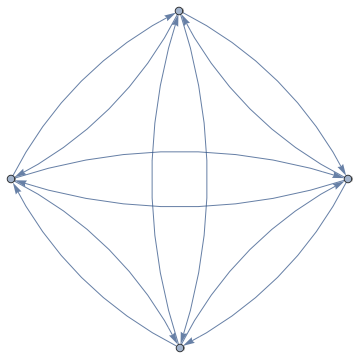
\includegraphics[width=0.5\textwidth]{grafo.pdf}
\caption[Grafo]{Grafo gris.}
\label{imagen:grafo}
\end{figure}

\begin{figure}[h!]
\centering
\includegraphics[width=\textwidth]{grafocolor.pdf}
\caption[Grafo coloreado (esto sale en la tabla de contenidos)]{Grafo con color.}
\label{imagen:grafodecolores}
\end{figure}

\chapter{@nombreApendice}
\label{apendiceB}
\lhead{Apéndice B. \emph{@nombreApendice}}

\Blindtext

\addtocontents{toc}{\vspace{2em}}

\backmatter

\end{document}
